\documentclass[10pt,a4paper]{article}
\usepackage[margin=1.9cm]{geometry}
\usepackage{booktabs}
\usepackage{graphicx}
\usepackage{amsmath}
\usepackage{caption}
\usepackage{enumitem}
\usepackage{float}
\usepackage[T1]{fontenc}
\usepackage{lmodern}
\usepackage{microtype}
\captionsetup{font=small,skip=3pt}
\setlist{itemsep=1pt,topsep=2pt,leftmargin=*}
\setlength{\parskip}{3pt}
\setlength{\parindent}{0pt}
\renewcommand{\arraystretch}{1.05}

\title{\vspace{-1.2cm}\textbf{Parameter-Efficient Fine-Tuning for Urdu Fake News Detection}\\[2pt]
\large Generative AI, Assignment 3 \quad Group 8 (Track 4) \quad Seeds 8 and 108\vspace{-0.4cm}}
\author{}
\date{}

\begin{document}
\maketitle

\section{Setup}
We compare Full Fine-Tuning (FT), LoRA, QLoRA and IA$^3$ on \texttt{community-datasets/urdu\_fake\_news} (Track 4, Real vs Fake) with \texttt{xlm-roberta-base} and \texttt{google/muril-base-cased}. All runs used one GTX 1070 (8 GB) with fp16 mixed precision. The PDF lists the dataset as \texttt{communitydatasets/...}; the working Hub name has a hyphen.

\begin{table}[H]
\centering\small
\begin{tabular}{@{}lp{13.3cm}@{}}
\toprule
Data & 900 articles (the given train and test parts merged), 2 classes. No empty rows were found; 6 exact duplicates were removed, leaving 894 articles. Stratified 70/15/15 split with seed 8 (fixed for all runs). \\
Cleaning & (1) strip whitespace and drop empty rows; (2) drop exact duplicates; (3) remove URLs and @mentions; (4) unify Arabic yeh (U+064A, U+0649) to Urdu yeh (U+06CC), Arabic kaf (U+0643) to Urdu kaf (U+06A9) and Arabic heh (U+0647) to Urdu heh (U+06C1); (5) remove diacritics and tatweel; (6) collapse repeated whitespace. \\
Length & max\_length 512. The 95th percentile of token length is 1070 (XLM-R) and 979 (MuRIL), above the 512-token limit of both models, so we use 512 and accept truncation of the tail of long articles. \\
Training & AdamW, linear schedule, 10\% warmup, weight decay 0.01, per-device batch 4 with 4 accumulation steps (effective 16), fp16, \textbf{10 epochs}, learning rate $2\times10^{-5}$ (Full FT) and $2\times10^{-4}$ (PEFT). Metrics are measured on the test split after the last epoch. \\
LoRA/QLoRA & $\alpha=16$, dropout 0.05, \texttt{task\_type=SEQ\_CLS}. ``attn'' = query and value; ``attn+FF'' adds the intermediate and output dense layers of each block. QLoRA: 4-bit NF4, double quantization, fp16 compute, \texttt{prepare\_model\_for\_kbit\_training}; the classifier is kept unquantized. \\
IA$^3$ & Vectors on key and value (attn) or key, value and the FF output layer (attn+FF); classifier head trained. \\
\bottomrule
\end{tabular}
\caption{Experimental setup. Deviation from the brief: 10 epochs instead of 3 (see Section 4).}
\end{table}

\begin{table}[H]
\centering\small
\begin{minipage}[t]{0.42\textwidth}\centering
\begin{tabular}{@{}lrrr@{}}
\toprule
Split & Fake & Real & Total \\
\midrule
train & 279 & 346 & 625 \\
val & 60 & 74 & 134 \\
test & 60 & 75 & 135

\\
\bottomrule
\end{tabular}
\caption{Class distribution.}
\end{minipage}\hfill
\begin{minipage}[t]{0.56\textwidth}\centering
\begin{tabular}{@{}lrrrr@{}}
\toprule
Tokenizer & Fertility & P95 & Trunc.\ \% & UNK \% \\
\midrule
xlm-roberta-base & 1.295 & 1070 & 25.0 & 0.0004 \\
google/muril-base-cased & 1.195 & 979 & 21.9 & 0.0230

\\
\bottomrule
\end{tabular}
\caption{Tokenizer analysis on the training split. Fertility is subword tokens per whitespace word; truncation is the share of texts longer than 512 tokens.}
\end{minipage}
\end{table}

\section{Main results}
Mean $\pm$ standard deviation over seeds 8 and 108 (sample standard deviation, $n=2$). Exp 04 is the attn+FF variant (the attn-only variant is Exp 03); 07a is IA$^3$ attn and 07b is attn+FF; 06 is QLoRA without paged AdamW. Exp 08 uses the best configuration of each method by validation macro-F1: Full FT (01), LoRA (04), QLoRA (05), IA$^3$ (07a). Memory is peak allocated GPU memory; params are trainable parameters in millions. A macro-F1 of 0.357 equals always predicting the majority class.

\begin{table}[H]
\centering\footnotesize
\begin{tabular}{@{}llccccr@{}}
\toprule
Exp & Configuration & Macro-F1 & Accuracy & Time (s) & Mem (GB) & Params (M) \\
\midrule
01 & Full FT & 0.654 $\pm$ 0.022 & 0.678 $\pm$ 0.037 & 652 $\pm$ 1 & 5.24 $\pm$ 0.00 & 278.045 \\
02 & LoRA r=8, attn & 0.515 $\pm$ 0.054 & 0.607 $\pm$ 0.052 & 479 $\pm$ 1 & 1.89 $\pm$ 0.00 & 0.887 \\
03 & LoRA r=16, attn & 0.541 $\pm$ 0.013 & 0.622 $\pm$ 0.021 & 480 $\pm$ 0 & 1.90 $\pm$ 0.00 & 1.182 \\
04 & LoRA r=16, attn+FF & 0.557 $\pm$ 0.146 & 0.641 $\pm$ 0.068 & 543 $\pm$ 0 & 2.23 $\pm$ 0.00 & 2.657 \\
05 & QLoRA r=16, paged & 0.467 $\pm$ 0.155 & 0.567 $\pm$ 0.016 & 527 $\pm$ 1 & 1.59 $\pm$ 0.00 & 1.182 \\
06 & QLoRA r=16, not paged & 0.471 $\pm$ 0.161 & 0.570 $\pm$ 0.021 & 526 $\pm$ 2 & 1.60 $\pm$ 0.00 & 1.182 \\
07a & IA3 attn & 0.357 $\pm$ 0.000 & 0.556 $\pm$ 0.000 & 472 $\pm$ 0 & 1.85 $\pm$ 0.00 & 0.611 \\
07b & IA3 attn+FF & 0.357 $\pm$ 0.000 & 0.556 $\pm$ 0.000 & 505 $\pm$ 1 & 2.17 $\pm$ 0.00 & 0.647 \\
08 & full (01), 25\% data & 0.357 $\pm$ 0.000 & 0.556 $\pm$ 0.000 & 166 $\pm$ 3 & 5.26 $\pm$ 0.00 & 278.045 \\
08 & full (01), 50\% data & 0.580 $\pm$ 0.004 & 0.607 $\pm$ 0.021 & 328 $\pm$ 2 & 5.25 $\pm$ 0.00 & 278.045 \\
08 & ia3 (07a), 25\% data & 0.357 $\pm$ 0.000 & 0.556 $\pm$ 0.000 & 121 $\pm$ 3 & 1.84 $\pm$ 0.00 & 0.611 \\
08 & ia3 (07a), 50\% data & 0.357 $\pm$ 0.000 & 0.556 $\pm$ 0.000 & 239 $\pm$ 2 & 1.85 $\pm$ 0.00 & 0.611 \\
08 & lora (04), 25\% data & 0.357 $\pm$ 0.000 & 0.556 $\pm$ 0.000 & 139 $\pm$ 3 & 2.21 $\pm$ 0.00 & 2.657 \\
08 & lora (04), 50\% data & 0.433 $\pm$ 0.108 & 0.570 $\pm$ 0.021 & 274 $\pm$ 2 & 2.21 $\pm$ 0.00 & 2.657 \\
08 & qlora (05), 25\% data & 0.357 $\pm$ 0.000 & 0.556 $\pm$ 0.000 & 135 $\pm$ 3 & 1.59 $\pm$ 0.00 & 1.182 \\
08 & qlora (05), 50\% data & 0.357 $\pm$ 0.000 & 0.556 $\pm$ 0.000 & 267 $\pm$ 2 & 1.59 $\pm$ 0.00 & 1.182

\\
\bottomrule
\end{tabular}
\caption{Results for XLM-R base.}
\end{table}

\begin{table}[H]
\centering\footnotesize
\begin{tabular}{@{}llccccr@{}}
\toprule
Exp & Configuration & Macro-F1 & Accuracy & Time (s) & Mem (GB) & Params (M) \\
\midrule
01 & Full FT & 0.467 $\pm$ 0.156 & 0.581 $\pm$ 0.037 & 635 $\pm$ 3 & 4.60 $\pm$ 0.00 & 237.558 \\
02 & LoRA r=8, attn & 0.357 $\pm$ 0.000 & 0.556 $\pm$ 0.000 & 476 $\pm$ 1 & 1.73 $\pm$ 0.00 & 0.296 \\
03 & LoRA r=16, attn & 0.357 $\pm$ 0.000 & 0.556 $\pm$ 0.000 & 477 $\pm$ 1 & 1.74 $\pm$ 0.00 & 0.591 \\
04 & LoRA r=16, attn+FF & 0.357 $\pm$ 0.000 & 0.556 $\pm$ 0.000 & 539 $\pm$ 3 & 2.06 $\pm$ 0.01 & 2.066 \\
05 & QLoRA r=16, paged & 0.357 $\pm$ 0.000 & 0.556 $\pm$ 0.000 & 516 $\pm$ 1 & 1.43 $\pm$ 0.01 & 0.591 \\
06 & QLoRA r=16, not paged & 0.357 $\pm$ 0.000 & 0.556 $\pm$ 0.000 & 513 $\pm$ 1 & 1.43 $\pm$ 0.01 & 0.591 \\
07a & IA3 attn & 0.357 $\pm$ 0.000 & 0.556 $\pm$ 0.000 & 469 $\pm$ 1 & 1.69 $\pm$ 0.00 & 0.020 \\
07b & IA3 attn+FF & 0.357 $\pm$ 0.000 & 0.556 $\pm$ 0.000 & 502 $\pm$ 0 & 2.01 $\pm$ 0.00 & 0.057 \\
08 & full (01), 25\% data & 0.357 $\pm$ 0.000 & 0.556 $\pm$ 0.000 & 162 $\pm$ 4 & 4.60 $\pm$ 0.00 & 237.558 \\
08 & full (01), 50\% data & 0.357 $\pm$ 0.000 & 0.556 $\pm$ 0.000 & 321 $\pm$ 3 & 4.60 $\pm$ 0.00 & 237.558 \\
08 & ia3 (07a), 25\% data & 0.357 $\pm$ 0.000 & 0.556 $\pm$ 0.000 & 120 $\pm$ 4 & 1.69 $\pm$ 0.00 & 0.020 \\
08 & ia3 (07a), 50\% data & 0.357 $\pm$ 0.000 & 0.556 $\pm$ 0.000 & 239 $\pm$ 1 & 1.69 $\pm$ 0.00 & 0.020 \\
08 & lora (04), 25\% data & 0.357 $\pm$ 0.000 & 0.556 $\pm$ 0.000 & 141 $\pm$ 1 & 2.05 $\pm$ 0.00 & 2.066 \\
08 & lora (04), 50\% data & 0.357 $\pm$ 0.000 & 0.556 $\pm$ 0.000 & 275 $\pm$ 1 & 2.06 $\pm$ 0.01 & 2.066 \\
08 & qlora (05), 25\% data & 0.357 $\pm$ 0.000 & 0.556 $\pm$ 0.000 & 132 $\pm$ 3 & 1.43 $\pm$ 0.00 & 0.591 \\
08 & qlora (05), 50\% data & 0.357 $\pm$ 0.000 & 0.556 $\pm$ 0.000 & 263 $\pm$ 1 & 1.43 $\pm$ 0.01 & 0.591

\\
\bottomrule
\end{tabular}
\caption{Results for MuRIL base.}
\end{table}

\section{Plots}
\begin{figure}[H]
\centering
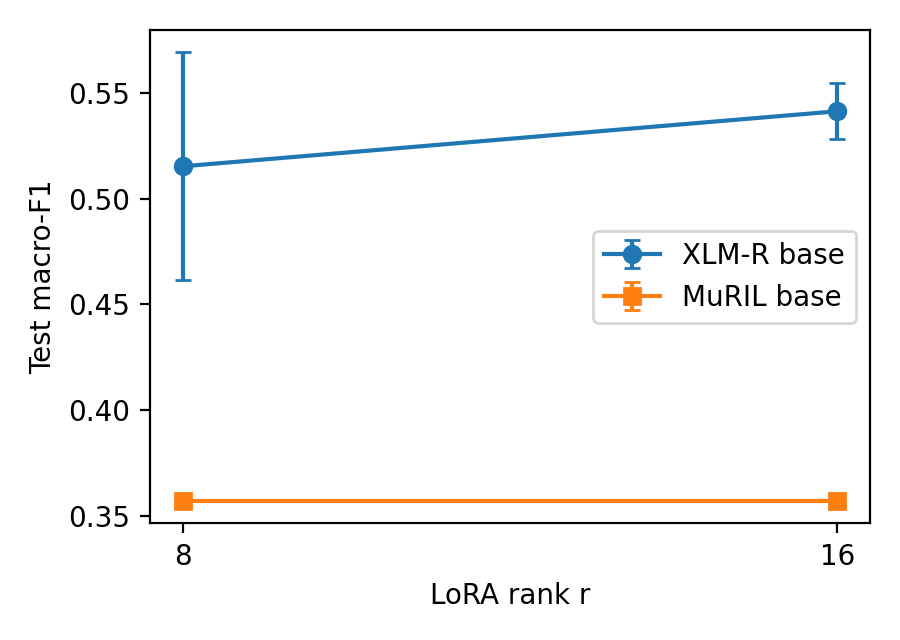
\includegraphics[width=0.47\textwidth]{plot_lora_rank.png}\hfill
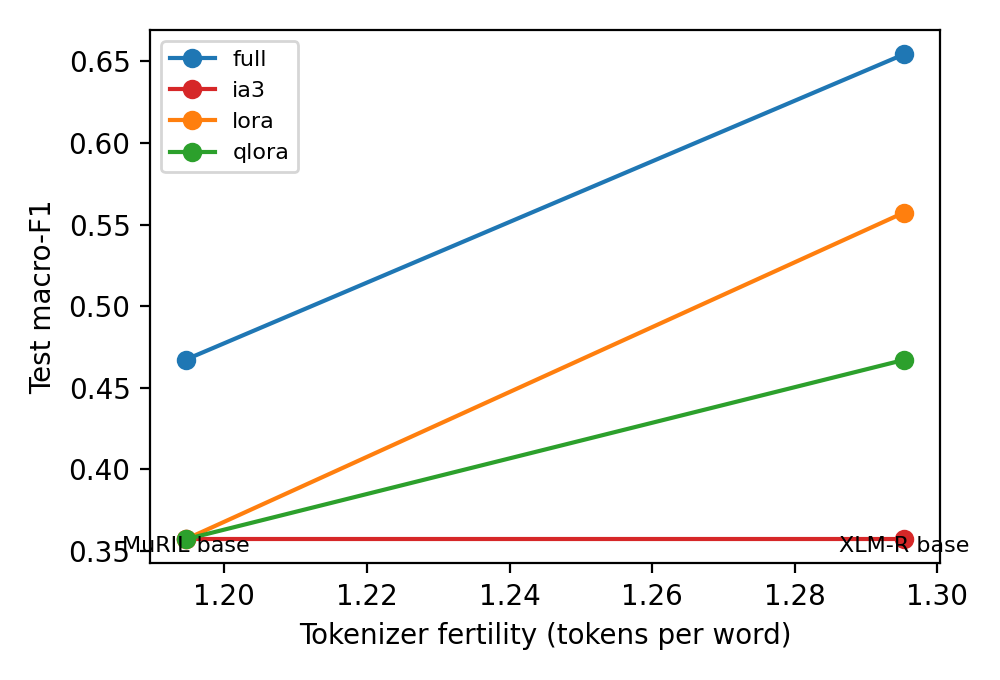
\includegraphics[width=0.47\textwidth]{plot_fertility.png}
\caption{Left: LoRA rank against macro-F1 (error bars are one standard deviation); MuRIL stays at chance for both ranks. Right: tokenizer fertility against macro-F1 for the best configuration of each method; the lower-fertility MuRIL scores lower.}
\end{figure}

\begin{figure}[H]
\centering
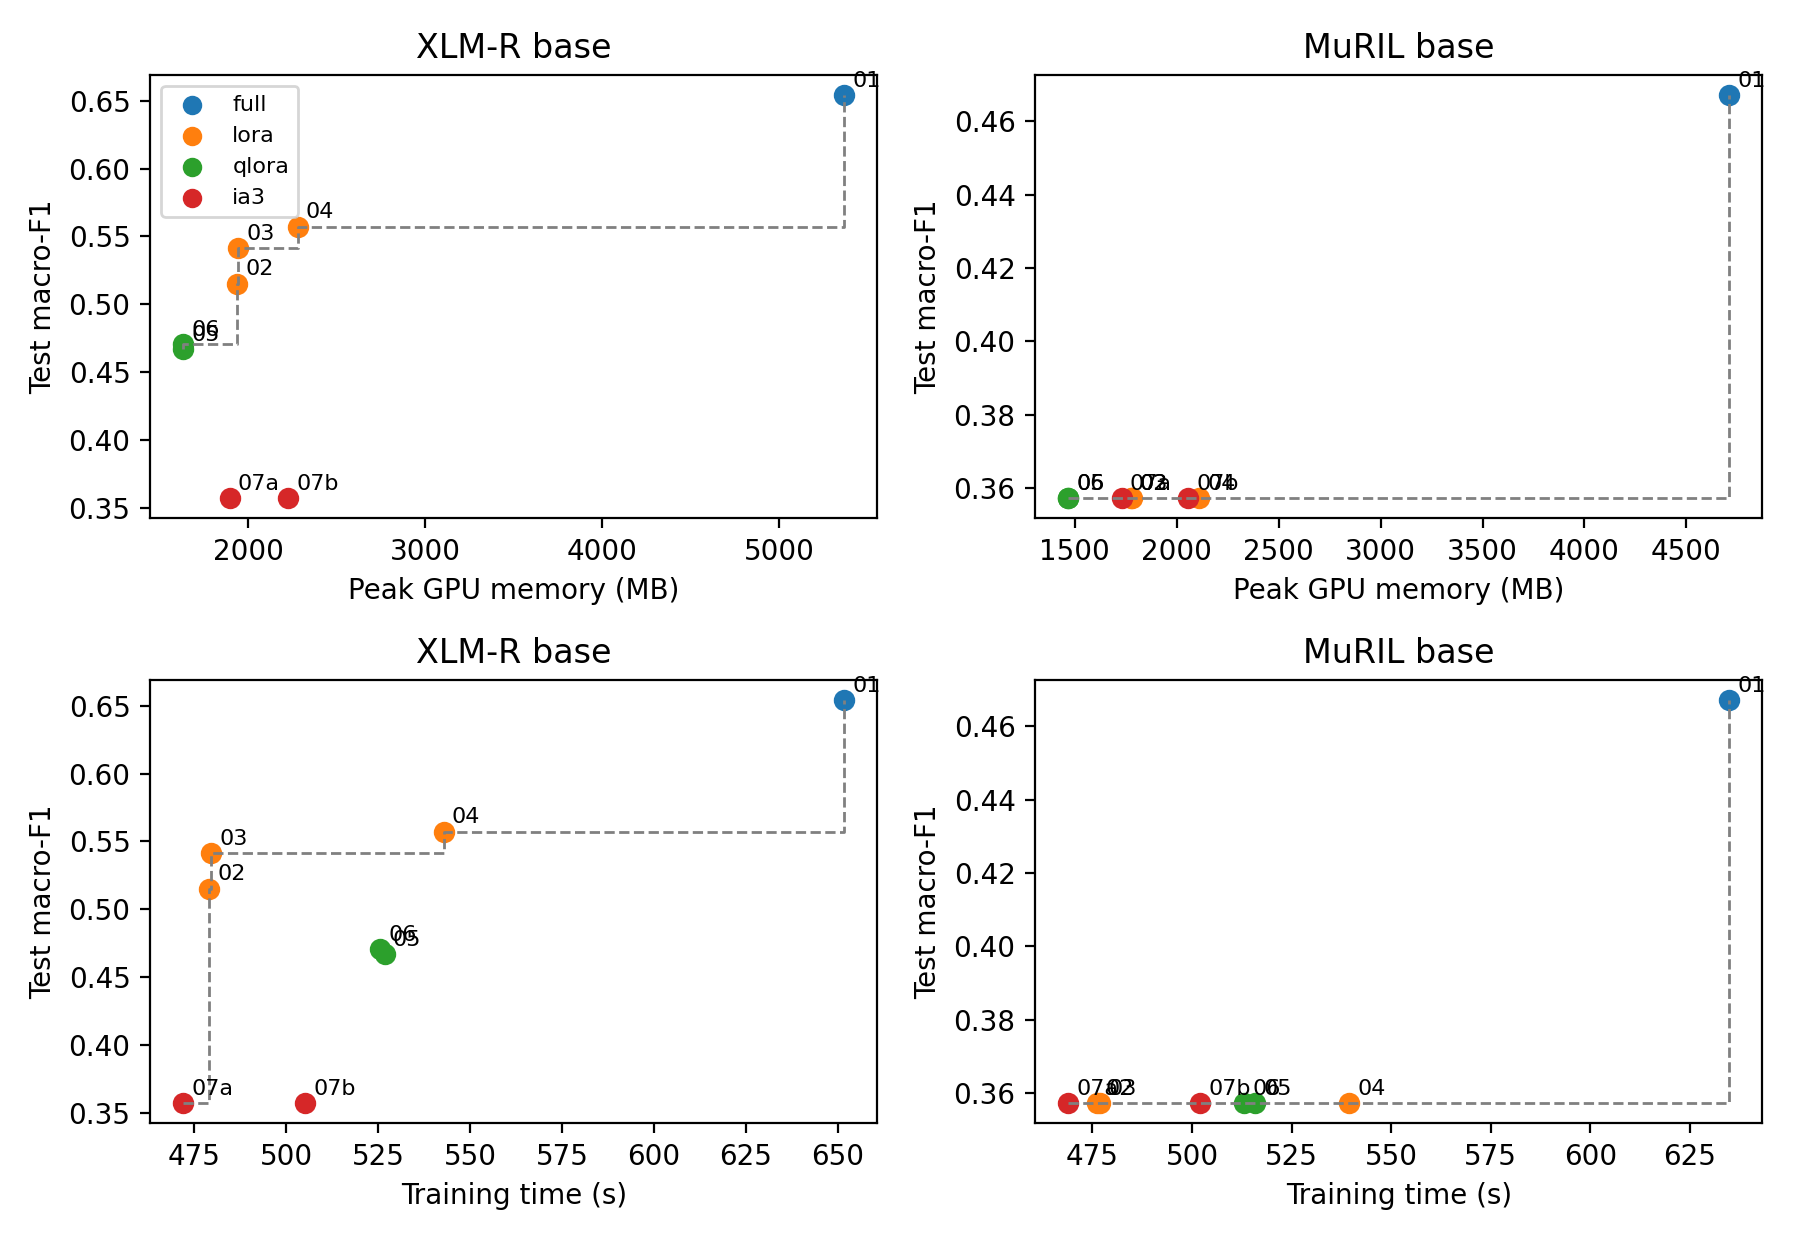
\includegraphics[width=0.78\textwidth]{plot_pareto.png}
\caption{Macro-F1 against peak GPU memory (top) and training time (bottom) for all configurations, with the Pareto front dashed.}
\end{figure}

\begin{figure}[H]
\centering
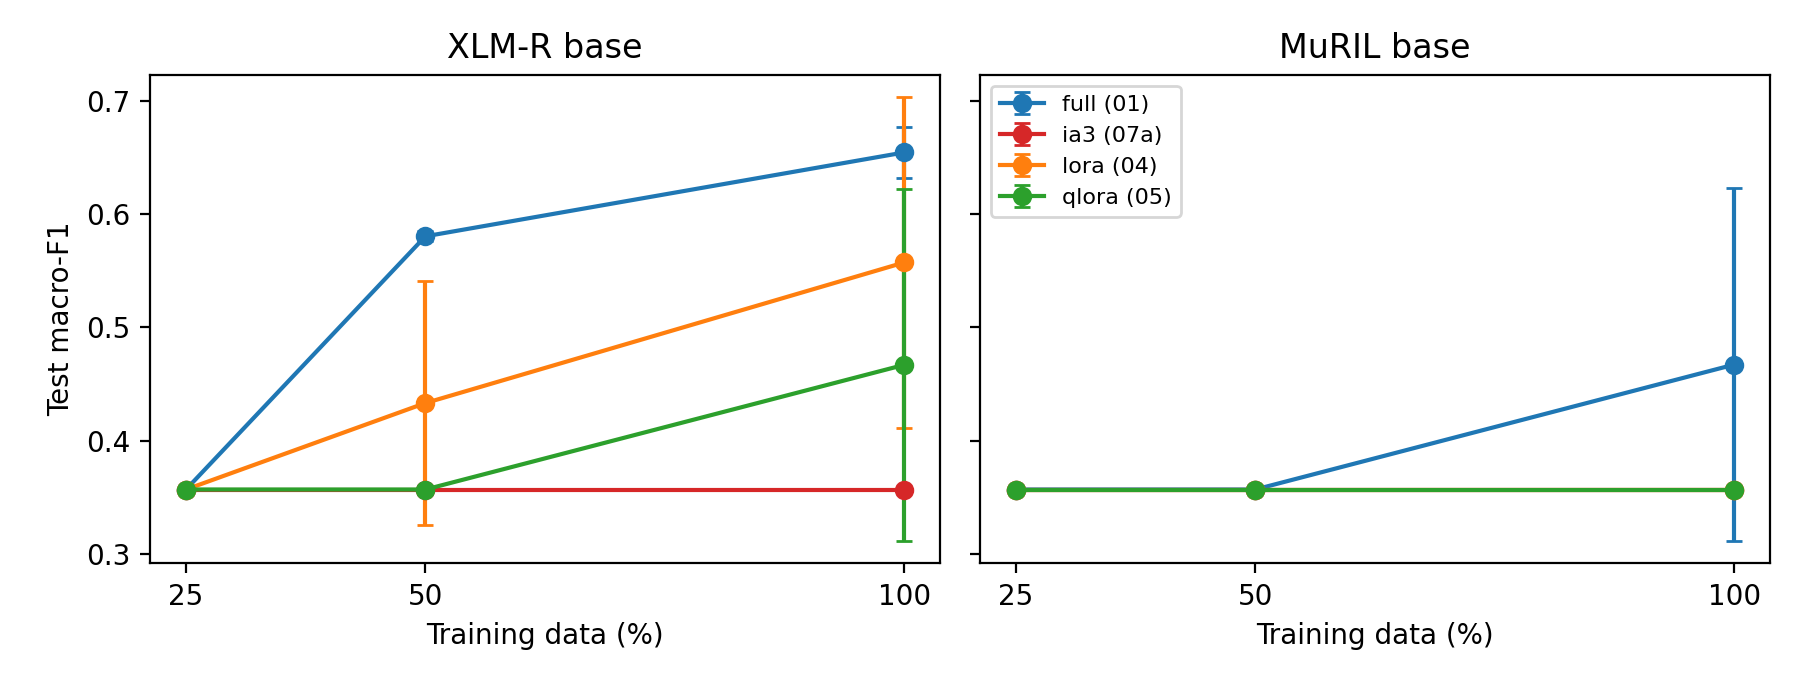
\includegraphics[width=0.78\textwidth]{plot_data_size.png}
\caption{Macro-F1 against training data size for the best configuration of each method. Methods at 0.357 are at chance level.}
\end{figure}

\section{Discussion}
\textbf{Why we used 10 epochs instead of 3.} We first ran the full grid exactly as specified (3 epochs, about 117 optimizer steps at an effective batch of 16 on 625 training articles). The result was unusable: 63 of the 64 runs scored exactly the majority-class macro-F1 of 0.357 (accuracy 0.556, the share of Real articles in the test split), for every method and both models (Table 6). The only exception was one MuRIL Full FT run at 25\% data (0.607), which is noise rather than learning. The logged training loss stayed at about $\ln 2$ per example throughout, so the models were not learning at all. We checked that the labels reach the loss and that fp32 and different warmup settings change nothing, so this is not a pipeline fault. The task itself is hard and small: the test split has 135 articles, and a TF-IDF plus logistic regression baseline on our splits reaches only 0.437 macro-F1. In a short diagnostic run, XLM-R began to leave the chance level with 10 epochs (0.616), so we reran the entire grid with 10 epochs ($\approx$390 steps) and kept every other setting from the brief (learning rates, batch size, max\_length, seeds). The 3-epoch results are kept in \texttt{run\_3epochs/} and are the reference for the specified setting. Even with 10 epochs, several configurations remain at chance, and with two seeds the standard deviations are rough estimates. Conclusions below are tentative.

\begin{table}[H]
\centering\footnotesize
\begin{tabular}{@{}llcccccc@{}}
\toprule
 & & \multicolumn{3}{c}{XLM-R base} & \multicolumn{3}{c}{MuRIL base} \\
\cmidrule(lr){3-5}\cmidrule(lr){6-8}
Exp & Configuration & Macro-F1 & Acc. & Time (s) & Macro-F1 & Acc. & Time (s) \\
\midrule
01 & Full FT & 0.357 $\pm$ 0.000 & 0.556 & 200 & 0.357 $\pm$ 0.000 & 0.556 & 196 \\
02 & LoRA r=8, attn & 0.357 $\pm$ 0.000 & 0.556 & 149 & 0.357 $\pm$ 0.000 & 0.556 & 146 \\
03 & LoRA r=16, attn & 0.357 $\pm$ 0.000 & 0.556 & 148 & 0.357 $\pm$ 0.000 & 0.556 & 146 \\
04 & LoRA r=16, attn+FF & 0.357 $\pm$ 0.000 & 0.556 & 166 & 0.357 $\pm$ 0.000 & 0.556 & 165 \\
05 & QLoRA r=16, paged & 0.357 $\pm$ 0.000 & 0.556 & 160 & 0.357 $\pm$ 0.000 & 0.556 & 157 \\
06 & QLoRA r=16, not paged & 0.357 $\pm$ 0.000 & 0.556 & 161 & 0.357 $\pm$ 0.000 & 0.556 & 155 \\
07a & IA3 attn & 0.357 $\pm$ 0.000 & 0.556 & 142 & 0.357 $\pm$ 0.000 & 0.556 & 141 \\
07b & IA3 attn+FF & 0.357 $\pm$ 0.000 & 0.556 & 155 & 0.357 $\pm$ 0.000 & 0.556 & 152

\\
\bottomrule
\end{tabular}
\caption{Reference run with the specified 3 epochs (100\% data, mean $\pm$ std over two seeds). Every configuration predicts only the majority class. All data-size runs of this setting were also at 0.357, except MuRIL Full FT at 25\% data (0.482 $\pm$ 0.176).}
\end{table}

\begin{figure}[H]
\centering
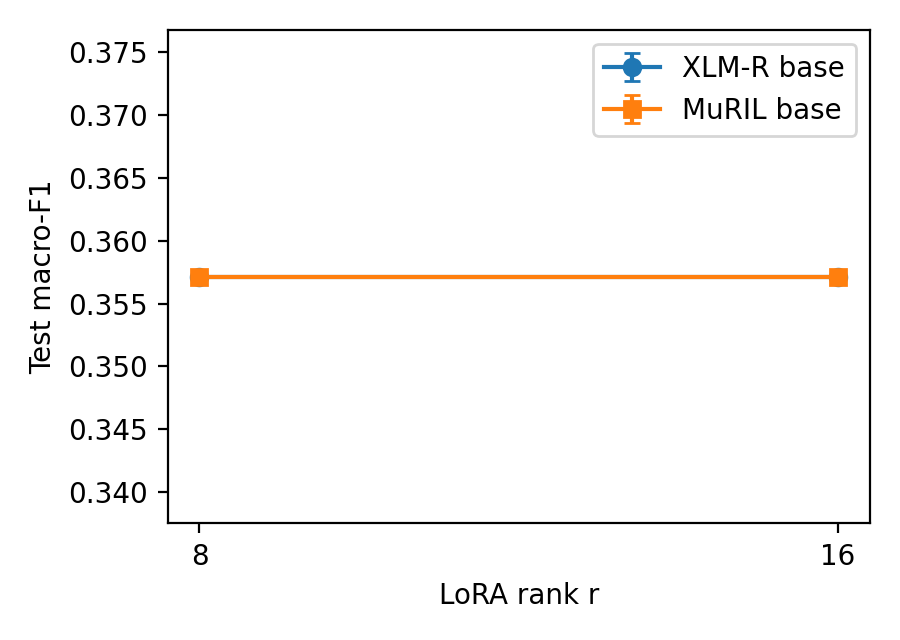
\includegraphics[width=0.47\textwidth]{run_3epochs/plot_lora_rank.png}\hfill
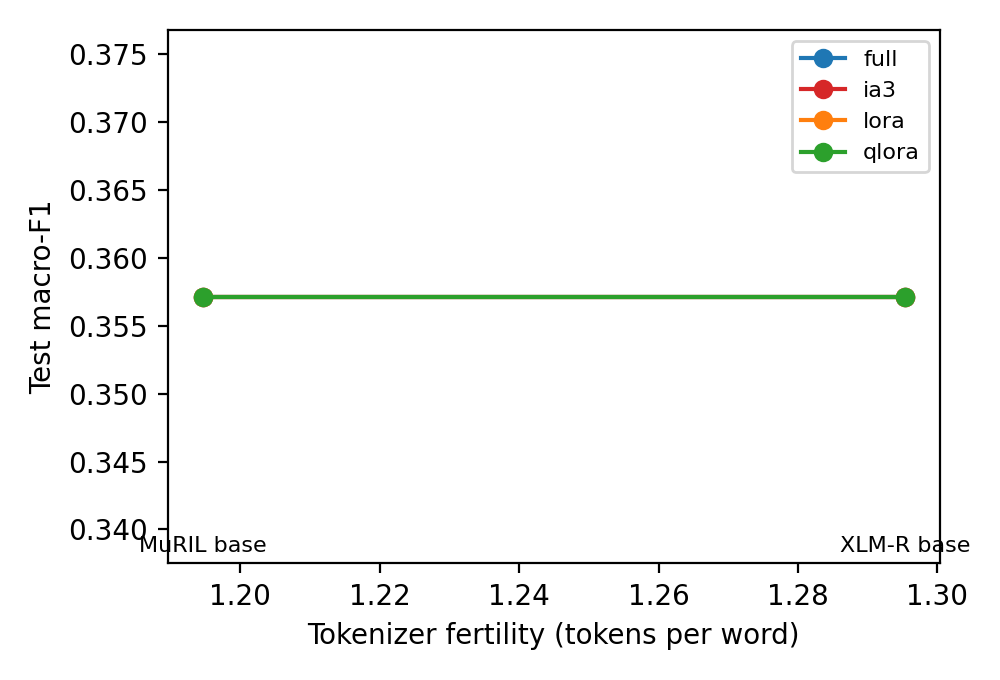
\includegraphics[width=0.47\textwidth]{run_3epochs/plot_fertility.png}
\caption{3-epoch reference run. Left: LoRA rank against macro-F1, a flat line at the majority-class score for both models. Right: fertility against macro-F1, again flat for every method.}
\end{figure}

\begin{figure}[H]
\centering
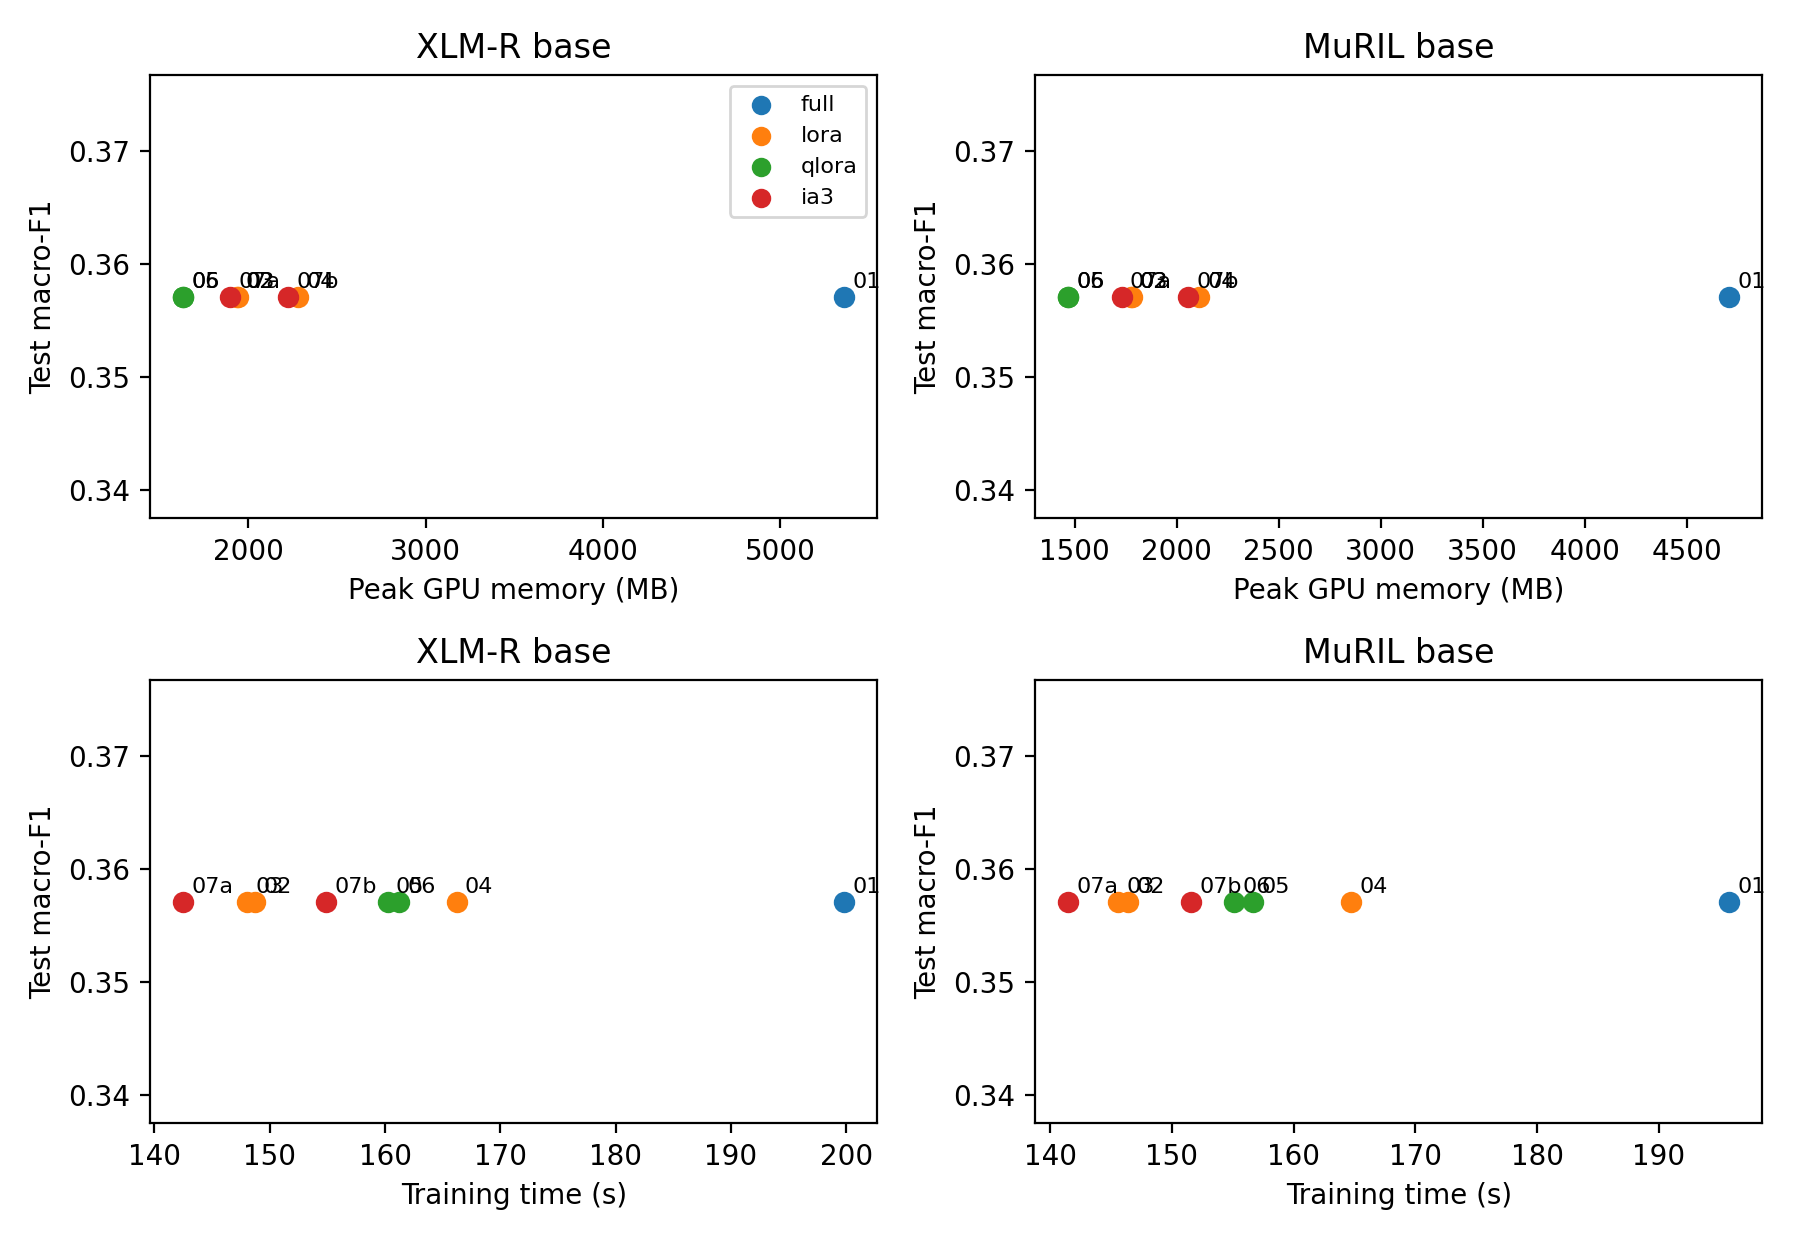
\includegraphics[width=0.7\textwidth]{run_3epochs/plot_pareto.png}
\caption{3-epoch reference run. Macro-F1 against peak memory (top) and training time (bottom): all configurations sit on one horizontal line, so there is no accuracy trade-off to read.}
\end{figure}

\begin{figure}[H]
\centering
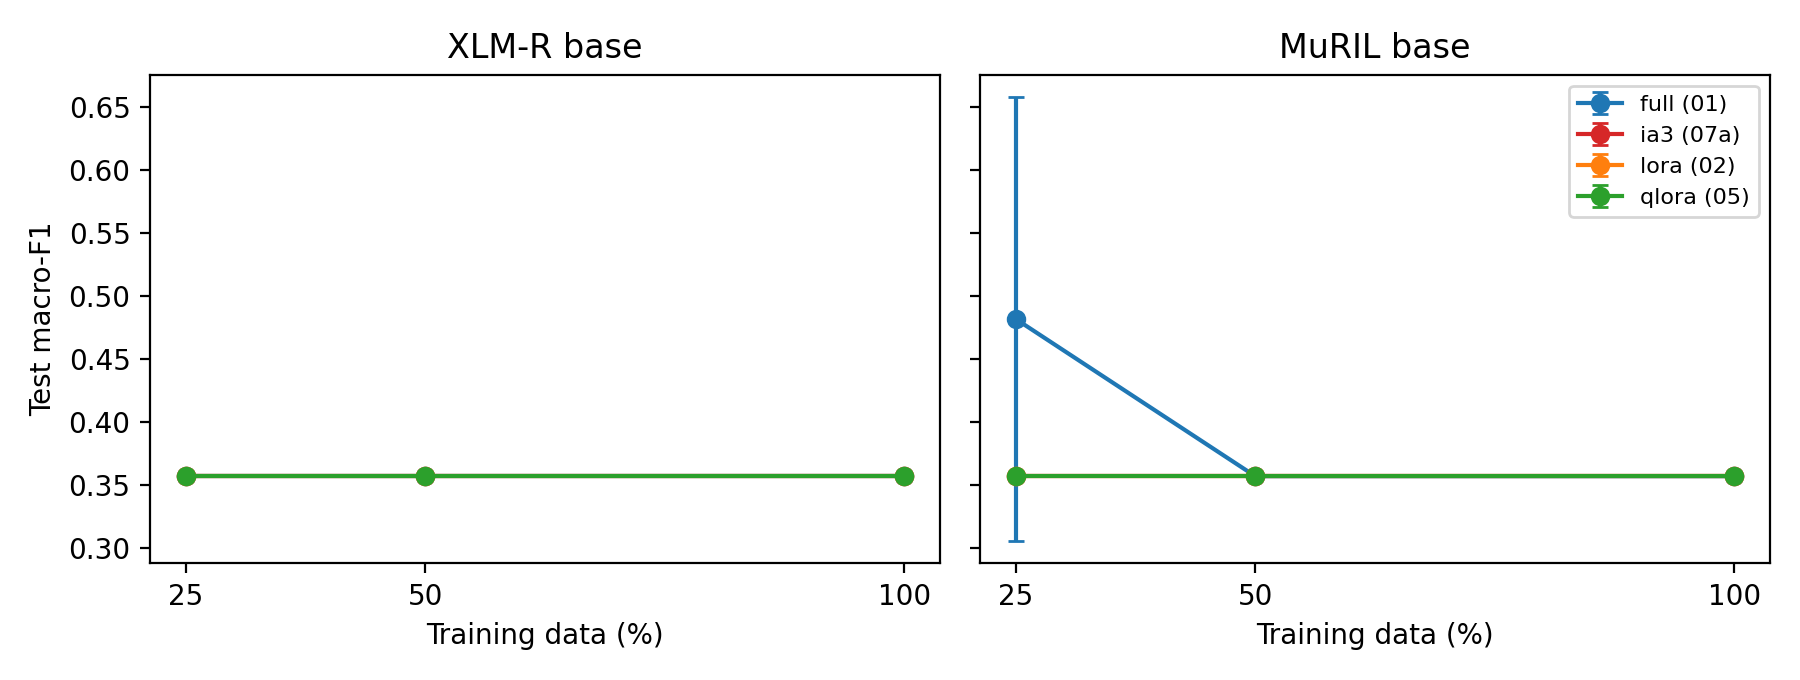
\includegraphics[width=0.7\textwidth]{run_3epochs/plot_data_size.png}
\caption{3-epoch reference run. Macro-F1 against training data size: flat at 0.357 except one MuRIL Full FT point at 25\% data.}
\end{figure}

\textbf{RQ1: accuracy against parameters, time and memory.} On XLM-R, Full FT is the most accurate (0.654) but costs 278M trainable parameters, 5.24 GB and 652 s. LoRA r=16 (attn) reaches 0.541, about 83\% of the Full FT score, with 1.18M parameters (0.4\%), 1.90 GB (36\% of Full FT) and 480 s (74\%). QLoRA (0.467) and IA$^3$ (0.357, chance) are cheaper still but clearly less accurate. The Pareto plots show Full FT, LoRA 04, LoRA 03, LoRA 02 and QLoRA as the non-dominated XLM-R points. The best accuracy-cost trade-off is LoRA r=16 (Exp 03); QLoRA is the choice when memory is the hard limit. On MuRIL only Full FT is above chance (0.467 with a large spread, std 0.156), so no trade-off can be read there. Note that IA$^3$ trains only the scaling vectors plus the classifier head, and at lr $2\times10^{-4}$ it did not leave the chance plateau; the learning rate is probably too low for it, but we did not tune it because the brief fixes it.

\textbf{Is r=16 worth its cost over r=8?} On XLM-R, r=16 scores 0.541 against 0.515 for r=8, at the same time (480 s) and the same memory (1.90 GB) and 0.3M more parameters. The gain is smaller than the seed spread (std 0.054 and 0.013), so it is weak evidence, but the extra cost is negligible, so r=16 is the safer choice.

\textbf{Do the feed-forward layers help?} Attn+FF gives 0.557 against 0.541 (attn only), a small mean gain with a very large seed spread (std 0.146), for 2.2$\times$ the parameters, +0.33 GB (2.23 vs 1.90 GB) and +63 s. We cannot call this a reliable improvement. On MuRIL neither variant left chance level.

\textbf{How much memory does QLoRA save, and at what cost?} Against LoRA r=16 attn on XLM-R, QLoRA lowers peak memory from 1.90 to 1.59 GB (16\% less), slows training by about 10\% (527 s against 480 s, from dequantization) and loses about 0.07 macro-F1 (0.467 against 0.541), with a large seed spread. Paged AdamW made no measurable difference (0.467 against 0.471; same memory and time), which is expected because our small optimizer state never needed to be paged out.

\textbf{RQ2: tokenizers.} MuRIL has lower fertility (1.195 against 1.295 tokens per word), a lower truncation rate (21.9\% against 25.0\%) and a higher unknown-token rate (0.023\%, against 0.0004\% for the SentencePiece XLM-R vocabulary). So MuRIL needs about 8\% fewer tokens for the same text, which explains only a small cost gap (Full FT 635 s against 652 s; most of the memory gap, 4.60 against 5.24 GB, comes from the smaller vocabulary and model, 237M against 278M parameters). Despite the better tokenization, MuRIL is less accurate here (Figure 1, right). With two models, fertility cannot be separated from other differences, so we do not claim that fertility drives accuracy; on this dataset it did not help.

\textbf{RQ3: scarce data.} With 25\% of the data, every method on both models is at chance. With 50\%, only Full FT on XLM-R is clearly above chance (0.580, against 0.654 at 100\%); LoRA gives 0.433 (high spread), QLoRA and IA$^3$ stay at chance, and MuRIL stays at chance for all methods. Full FT is therefore the most robust method when labelled data is scarce, and it degrades least (a drop of 0.07 from 100\% to 50\%), while the PEFT methods lose their signal first. This agrees with the common observation that the small, randomly initialised PEFT modules and the classifier need more updates than the roughly 390 optimizer steps of 10 epochs on this dataset.

\section{Contributions}
The work was split evenly between two pairs.
\begin{itemize}
\item Hashir Rauf (23L-2572) and Abdul Moiz (23L-2632) completed one half of the assignment.
\item Saad Nasir (23L-2625) and Ibrahim Moeed (23L-2602) completed the other half.
\end{itemize}

\end{document}
